Randomized and approximation algorithms can obtain significant benefits from
coordination directives because their inherent non-determinism can be harnessed
to evaluate rules in different orders.
An example of such program is Loopy Belief Propagation~(LBP).
LBP~\cite{Murphy99loopybelief} is an approximate inference algorithm
used in graphical models with cycles. In its essence, LBP is a sum-product message passing algorithm
where nodes exchange messages with their immediate neighbors and apply some computations to the messages
received.

LBP maps very well to the graph based model of CLM. In its
original form, the belief values of nodes are computed by synchronous iterations.
LBP offers more concurrency when belief values are computed asynchronously
leading to faster convergence. For this, every node keeps track of all messages
sent/received and recomputes the belief using partial information from neighbor
nodes. It is then possible to prioritize the computation of beliefs when a
neighbor's belief changes significantly.

The asynchronous approach proves to be a nice improvement over the synchronous
version. Still, it is possible to do even better. Gonzalez et
al~\cite{Gonzalez+al:aistats09paraml} developed an optimal algorithm to compute
this algorithm by first building a tree and then updating the beliefs of each
node twice, first from the leaves to the root and then from the root to the
leaves. The root of this tree is the node with the highest priority (based on
belief) while the other nodes in the tree must have a non-zero priority.
Note that the priorities are updated whenever a neighbor updates their belief.
These \emph{splash trees} are built iteratively until we reach convergence.
%In Fig.~\ref{splash_bp} we represent two threads creating two different splash trees.

\iffalse
\begin{topfig}
   \begin{center}
      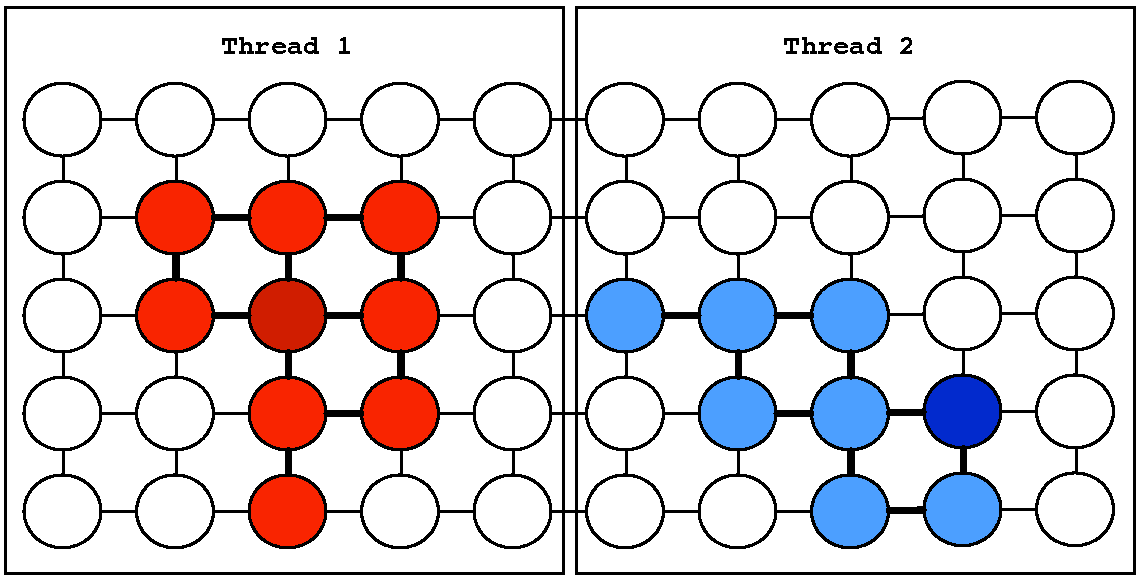
\includegraphics[width=6.5cm]{figures/splash_bp}
   \end{center}
   \scap{splash_bp}{Creating splash trees for belief propagation. Each threads picks the
   highest priority node and creates a tree from that node. The belief values
   are updated in two phases: first from the leaves to the root and then from
   the root to the leaves.}
\end{topfig}
\fi

The code for Splash Belief Propagation~(SBP) in Fig.~\ref{code:sbp} presents the
coordination code for LBP.  Please note that we just appended the code in
Fig.~\ref{code:sbp} to a working but unoptimized version of the algorithm, every
other rule remains the same. We added new rules that coordinate
the creation and execution of the splash trees:

\begin{tightdescription}
   \item[Tree building]: Each node has a \mytt{inactive} fact that is used to
   start the tree building process. When the highest priority node is picked, a
   \mytt{tree} is created that will navigate through the tree. In lines 15-21,
   we use an \emph{aggregate}~\cite{cruz-iclp14} to gather all the neighbor
   nodes that have a positive priority (due to a new belief update) and are in the
   same thread. Nodes are collected into list \mytt{L} and
   appended to list \mytt{Next} (line 21).
   
   \item[First phase]: When the number of nodes in the tree reaches a certain
   limit, a \mytt{first-phase} (lines 11-12) is generated to update the beliefs of
   all nodes in the tree. As the nodes are updated, starting from the leaves and
   ending at the root, an \mytt{update} fact is derived to update the belief
   values (line 35).

   \item[Second phase]: In the second phase, the computation of beliefs is
   performed from the root to the leaves and the belief values are updated a
   second time (line 42).
\end{tightdescription}

The \mytt{set-static} and \mytt{set-cpu} action facts are used in
line 2 to (1) force nodes to stay in the thread and (2) 
partition nodes as a grid of threads. This sets up well defined areas
of nodes for threads to build splash trees on.

\begin{topfig}
\scriptsize\begin{Verbatim}[numbers=left,commandchars=*\{\}]
!coord(A, X, Y), start(A)
   -o *underline{set-static(A), set-cpu(A, grid(X, Y))}.

// TREE BUILDING: expand tree by adding nodes
inactive(A), tree(A, All, Next)
   -o expand-tree(A, All, Next).
// start tree since we do not have one
inactive(A), *underline{@priority(A, A, P)}, P > 0.0
   -o expand-tree(A, [A], [A]).
// end tree building
expand-tree(A, All, Next), len(All) >= maxnodes
   -o first-phase(A, All, reverse(All)).
// expand tree
expand-tree(A, All, [A | Next]), len(Next) < maxnodes-1
   -o [collect => L | Side | !edge(A, L, Side),
         0 = count(All, L), // L is not in All
         0 = count(Next, L), // L is not in Next
         *underline{@priority(A, L, P), P > 0.0,}
         *underline{@cpu-id(A, L, Id1)},
         *underline{@cpu-id(A, A, Id2), Id1 = Id2} |
         send-tree(A, All, Next ++ L)].

send-tree(A, All, [])
   -o first-phase(A, All, reverse(All)).
send-tree(A, All, [B | Next])
   -o *underline{schedule-next(B)},
      tree(B, All ++ [B], [B | Next]).

// FIRST PHASE
first-phase(A, [A], [A]) -o second-phase(A, [], A).
first-phase(A, [A, B | Next], [A])
   -o update(A), *underline{schedule-next(B)},
      second-phase(B, [B | Next], A).
first-phase(A, All, [A, B | Next])
   -o update(A), *underline{schedule-next(B)},
      first-phase(B, All, [B | Next]).

// SECOND PHASE
second-phase(A, [], _)
   -o *underline{remove-priority(A)}, inactive(A), update(A).
second-phase(A, [A], Back)
   -o update(A), inactive(Back),
      inactive(A), *underline{remove-priority(A)}.
second-phase(A, [A, B | Next], Back)
   -o update(A), inactive(Back), *underline{schedule-next(B)},
      second-phase(B, [B | Next], A).
\end{Verbatim}
  \scap{code:sbp}{Coordination code for the Splash Belief Propagation program. 
%CLM needs 50 lines of rules to implement splash trees, while GraphLab needs a total of 350 lines of C++ to implement the same functionality.
  Note
     that when a linear fact is prefixed by \mytt{@}, it indicates that the
     fact is going to be re-derived.}
\end{topfig}
\normalsize

\begin{dblfig}
\vspace*{-1ex}
   \begin{center}
      \subfloat[]{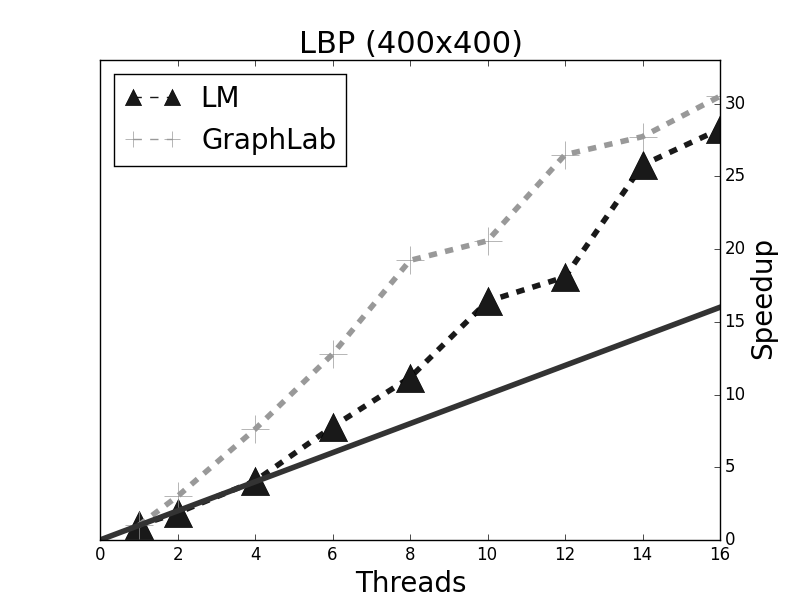
\includegraphics[width=\figsize]{results/system_belief-propagation-400.png}}
      \subfloat[]{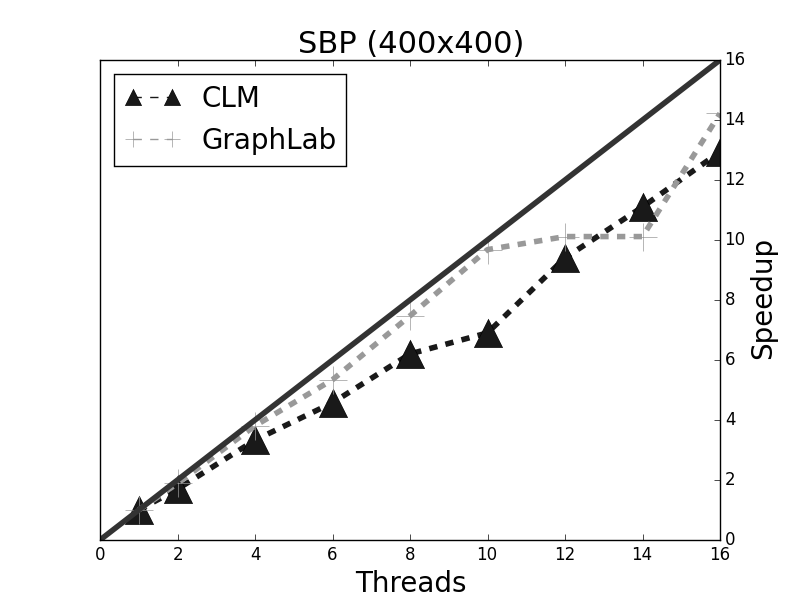
\includegraphics[width=\figsize]{results/system_splash-bp-400.png}}
      \subfloat[]{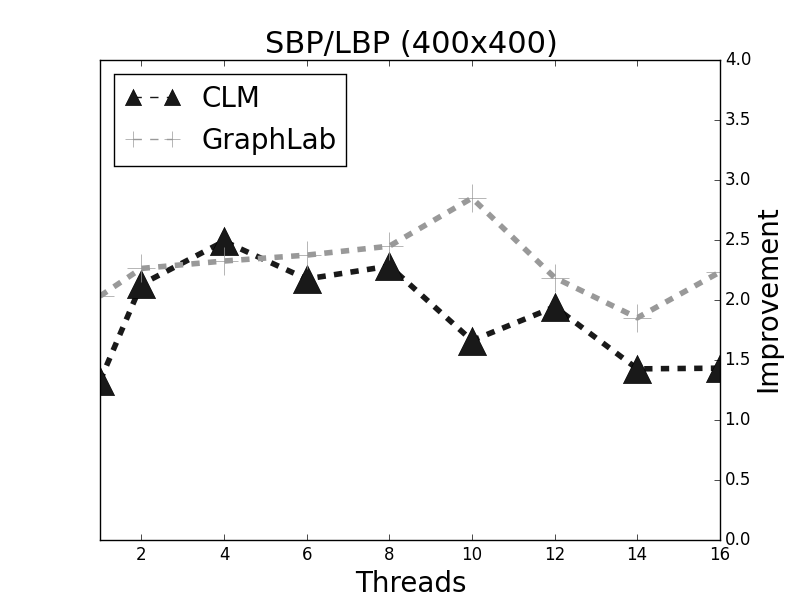
\includegraphics[width=\figsize]{results/system_improve_belief-propagation-400.png}}
   \end{center}
   \scap{results:splash_bp}{Experimental results for LBP and SBP. (a) shows the
      scalability of LBP for both CLM and GraphLab and (b) shows the
      scalability of SBP. (c) presents the
      improvements seen in SBP against LBP, where SBP runs, on average, 1.5 to 2.5
      times faster than LBP.}
\vspace*{-1ex}
\end{dblfig}

In this program, coordination assumes a far more important role than
we have seen before. Coordination rules drive the behavior of the
algorithm and while the result of the algorithm is statistically
identical to the original algorithm, SBP works very differently than
LBP.  SBP is also implemented in GraphLab~\cite{GraphLab2010}, a C++
framework for writing machine algorithms.  GraphLab provides the
splash scheduler as part of its the framework. It includes 350 lines
of C++ code.  With our coordination facts, it is possible to create
the necessary scheduling with only 12 rules.

We measured the behavior of LBP and SBP for both CLM and GraphLab.
Fig.~\ref{results:splash_bp} shows that both systems have very similar behavior
when using a variable number of threads.  The differences in performance between
GraphLab and CLM comes mainly because GraphLab performs in-place updates of
neighbor belief values, while CLM compiler and runtime system perform na\"{i}ve
manipulation of facts by deriving rules. The in-place update could be generated
by the compiler using smarter compilation strategies.
